After compiling \dftfe{} as described in Section~\ref{sec:installation}, we have now two executables --- \verb|$dftfe_build_dir/release/real/dftfe| and \verb|$dftfe_build_dir/release/complex/dftfe|. The \verb|$dftfe_build_dir/release/real/dftfe| executable, which uses real data-structures is sufficient for fully non-periodic problems. The executable can also be used for periodic and semi-periodic problems involving a Gamma point calculation. On the other hand the \verb|$dftfe_build_dir/release/complex/dftfe| executable, which uses complex data-structures is required for periodic and semi-periodic problems with multiple k point sampling for Brillouin zone integration. These executables are to be used for a parallel run as follows:
\begin{verbatim}
  mpirun -n N ./dftfe parameterFile.prm
\end{verbatim}
to run with N processors. 
\subsection{Structuring the input file}
In the above, an input file with \verb|.prm| extension is used. This file contains input parameters as described in Section~\ref{sec:parameters}, which can be of multiple types (\verb|string, double, integer, bool etc.|). All input parameters are also conveniently indexed at the end of this manual in Section~\ref{sec:runtime-parameter-index-full}. As seen in Section~\ref{sec:parameters}, there are two types of parameters: {\bf Global parameters} and {\bf Parameters in section} \verb|A/B/..|. In {\bf Parameters in section} \verb|A/B/..|, \verb|A| refers to the primary subsection name, \verb|B| if present refers to a subsection inside \verb|A|, and so on. 

First, lets consider how to use a parameter named \verb|PARAMETER xyz| under {\bf Global parameters}. To set it to a value, say \verb|value|  in the  \verb|.prm| file, directly use
\begin{verbatim}
  set PARAMETER xyz=value
\end{verbatim}
Next consider a parameter named \verb|PARAMETER xyzA| under {\bf Parameters in section} \verb|A|. To set it to a value, say \verb|value|  in the  \verb|.prm| file, use 
\begin{verbatim}
subsection A
  set PARAMETER xyzA=value
end
\end{verbatim}
Finally, consider a nested parameter named  \verb|PARAMETER xyzAB| under {\bf Parameters in section} \verb|A/B|. To set it to a value, say \verb|value|  in the  \verb|.prm| file, use 
\begin{verbatim}
subsection A
  subsection B
    set PARAMETER xyzAB=value
  end
end
\end{verbatim}
Couple of final comments--- more than one parameter could be used inside the same \verb|subsection|. For example,
\begin{verbatim}
subsection A
  set PARAMETER SUBSECTION xyzA1=value1
  set PARAMETER SUBSECTION xyzA2=value2
  subsection B
    set PARAMETER SUBSUBSECTION xyzAB1=value1
    set PARAMETER SUBSUBSECTION xyzAB2=value2
  end
end
\end{verbatim}
Also the indentation used in the above examples is only for readability.
\subsection{Demo examples}
Now we will walk you through a few demo examples in the \verb|/demo/| folder. We refer to
\begin{verbatim}
https://github.com/dftfeDevelopers/dftfe-benchmarks.git
\end{verbatim}
repository for a comphrehensive list of accuracy and performance examples, which are designed to cover most of the capabilities of the DFT-FE code. Further, we note that the demo examples in the \verb|/demo/| folder do not cover all the input parameter options. To get full list of input parameters see Section~\ref{sec:parameters}. All input parameters are also conveniently indexed at the end of this manual in Section~\ref{sec:runtime-parameter-index-full}. 
\subsubsection{Example 1}\label{sec:example1}
Let us consider the first example given in the folder
\verb|/demo/ex1|, where we compute the ground state of the Nitrogen molecule using pseudopotential DFT calculations employing fully non-periodic boundary conditions.
There are two input parameter files-- parameterFile\_a.prm and parameterFile\_b.prm. parameterFile\_a.prm is
computing the ground-state and forces of the Nitrogen molecule while parameterFile\_b.prm additionally does atomic relaxation.

Below, we provide a step by step procedure on setting up the above input parameter files, doing a total energy and force convergence study with respect to finite-element mesh discretization, and finally doing the atomic relaxation of Nitrogen molecule.
\begin{enumerate}
\item The geometry of the Nitrogen molecule (${\rm N}_{2}$) system is set using input parameters under \verb|Geometry| subsection
\begin{verbatim}
subsection Geometry
  set NATOMS=2
  set NATOM TYPES=1
  set ATOMIC COORDINATES FILE      = coordinates.inp 
  set DOMAIN VECTORS FILE = domainVectors.inp
end
\end{verbatim}
where
\begin{itemize}		

\item \verb|NATOMS| is the total number of atoms, and \verb|NATOM TYPES| is the total number of atom types.
	
\item``domainVectors.inp'' (any other file name can be used), given as input to \verb|DOMAIN VECTORS FILE|,  is the external input file which lists the three domain vectors (in a.u) describing the
3D parallelepiped computational domain. For the current example we take a cubodial domain with 40 a.u as the edge length. 
Accordingly, the ``domainVectors.inp'' file is formatted as  
\begin{verbatim}
40.0 0.0 0.0
0.0 40.0 0.0
0.0 0.0 40.0
\end{verbatim}
wheres each row corresponds to a domain vector.
It is a requirement that the above vectors must form a right-handed coordinate system i.e. $(v1 \times v2)\cdot v3 >0$.

\item ``coordinates.inp'' (any other file name can be used), given as input to \verb|ATOMIC COORDINATES FILE|, is the name of an external input file present in the same workspace which lists the Cartesian coordinates of the atoms (in a.u.) with respect to origin at the center of the domain. For this example, ``coordinates.inp'' is described as 
\begin{verbatim}
7    5   -1.30000000E+00   0.00000000E+00   0.00000000E+00
7    5    1.30000000E+00   0.00000000E+00   0.00000000E+00
\end{verbatim}
where each line corresponds to ``atomic-charge valence-charge x y z''. Since this is a pseudopotential calculation, the valence-charge must correspond to the pseudopotential input, which we disuss in the later steps.

{\bf We require Cartesian coordinates for fully non-periodic simulation domain like above while fractional coordinates
are mandatory for periodic and semi-periodic simulation domain.}
\end{itemize}

\item Set the fully non-periodic boundary conditions for the problem using the subsection\\ \verb|Boundary conditions|
\begin{verbatim}	
subsection Boundary conditions
  set PERIODIC1                       = false
  set PERIODIC2                       = false
  set PERIODIC3                       = false
end
\end{verbatim}
where \verb|PERIODIC1/2/3| sets the periodicity along the first, second, and third domain vectors.
We note that \dftfe{} allows for arbitrary boundary conditions.

\item
Set the required DFT functional input parameters for pseudopotential calculation 	
\begin{verbatim}
subsection DFT functional parameters
  set EXCHANGE CORRELATION TYPE   = 4
  set PSEUDOPOTENTIAL CALCULATION = true
  set PSEUDOPOTENTIAL FILE NAMES LIST = pseudo.inp
end
\end{verbatim}
where
\begin{itemize}		
\item The choice of ``4'' for \verb|EXCHANGE CORRELATION TYPE| corresponds to ``GGA: Perdew-Burke-Ernzerhof
functional [PRL. 77, 3865 (1996)]'' functional. 
		
\item ``pseudo.inp'', given as input to \verb|PSEUDOPOTENTIAL FILE NAMES LIST| is an external file (any other file name can be used) in the same workspace, which contains the list of pseudopotential file names in \verb|UPF| format corresponding to the atom types involved in the calculations. The file is formatted as 
\begin{verbatim}
7 N.upf
\end{verbatim}
		where ``7'' is the atomic number of Nitrogen, and \verb|N.upf| is the Optimized Norm-Conserving Vanderbilt pseudopotential (ONCV) file obtained from \url{http://www.pseudo-dojo.org/}. {\bf Presently, we only support Norm-Conserving pseudopotential (Troullier-Martins, ONCV) files in \verb|UPF| format (version 2.0 or greater)}.
\end{itemize}

\item Set the input parameters for Self-Consistent field iterative procedure.
\begin{verbatim}
subsection SCF parameters
  set MIXING PARAMETER = 0.5
  set MAXIMUM ITERATIONS               = 40
  set TEMPERATURE                      = 500
  set TOLERANCE                        = 5e-5
  subsection Eigen-solver parameters
      set NUMBER OF KOHN-SHAM WAVEFUNCTIONS = 12
  end
end	
\end{verbatim}
where
\begin{itemize}		
\item ``0.5'' set for \verb|MIXING PARAMETER| is the mixing parameter to be used in the mixing scheme.
\item ``40'' set for \verb|MAXIMUM ITERATIONS| is the maximum number of iterations allowed in SCF iterative procedure.
\item ``500'' set for \verb|TEMPERATURE| is the Fermi-Dirac smearing temperature in Kelvin.
\item ``5e-5'' set for \verb|TOLERANCE| is the SCF stopping tolerance in terms of L2 norm of the electron-density
difference between two successive iterations.
\item ``12'' set for \verb|NUMBER OF KOHN-SHAM WAVEFUNCTIONS| is the Number of Kohn-Sham wavefunctions to be computed in the Eigen solve (using Chebyshev subspace iteration solve) for every SCF iteration step. This parameter is set inside the subsection \verb|Eigen-solver parameters|, which is nested within \verb|SCF parameters|.
\end{itemize}

\item As we are also computing the force on the atoms in this example, update the \verb|Geometry| subsection in the first step to
\begin{verbatim}
subsection Geometry
  set NATOMS=2
  set NATOM TYPES=1
  set ATOMIC COORDINATES FILE      = coordinates.inp 
  set DOMAIN VECTORS FILE = domainVectors.inp
  subsection Optimization
    set ION FORCE = true
  end
end
\end{verbatim}
where the \verb|ION FORCE| is set to true inside the nested subsection \verb|Optimization|. This computes and prints the forces on the atoms at the end of the ground-state solve.

\item 
\dftfe{} as mentioned before employs finite-element basis. These basis are piecewise polynomial functions. The three important FE discretization related parameters in \dftfe{}, which the user needs to set are the POLYNOMIAL ORDER, MESH SIZE AROUND ATOM, and ATOM BALL RADIUS.

First, the POLYNOMIAL ORDER sets the order of the piecewise continuous FE interpolating polynomial, with higher values affording faster convergence rates with respect to discretization. Default value is set to 6. Based on our numerical investigations, we recommend POLYNOMIAL ORDER=7 for soft pseudopotentials ($<$ 20 Ha plane-wave cutoff), POLYNOMIAL ORDER=6 for medium hard/very hard pseudpotentials, and POLYNOMIAL ORDER=5 for all-electron calculations to be most computationally efficient choices on both CPUs and GPUs.

Second, the MESH SIZE AROUND ATOM input parameter sets the size (in Bohr units) of the FE mesh element around the atoms. Mesh sizes away from the atoms and the intervening mesh adaptivity is heuristically set inside the code depending on the domain boundary conditions. The MESH SIZE AROUND ATOM is the most important parameter for the user to control in pseudopotential DFT calculations. This parameter is inversely related to the plane-wave cutoff in plane-wave based DFT codes. Smaller mesh sizes lead to lower discretization related errors, but at the cost of more degrees of freedom. Based on our numerical validation studies as will be demonstrated in many of the examples, we obtain chemical accuracy (~$10^{-4}$ Ha/atom in energy, ~$10^{-4}$ Ha/Bohr in ionic forces and ~$5 \times 10^{-6}$ Ha/Bohr$^3$ in cell stresses) using the following choice of discretization parameters: (POLYNOMIAL ORDER=7, MESH SIZE AROUND ATOM=1.5 --- 2.5) for soft pseudopotentials, and (POLYNOMIAL ORDER=6, MESH SIZE AROUND ATOM=0.5 --- 1.5) for medium hard/very hard pseudopotentials. We advice the users to use the above recommendations as starting choices only and always check the convergence of their quantity of interest with respect to MESH SIZE AROUND ATOM as described below for the current demo example. For all-electron calculations, a value of around 0.5 is a good starting choice. %(see examples 3 and 4).

Third, the ATOM BALL RADIUS input parameter denotes the radius of ball enclosing every atom (in a.u.), inside which the mesh size is set close to MESH SIZE AROUND ATOM and coarse-grained in the region outside the enclosing balls. For the default value of 0.0, a heuristically determined value is used, which is good enough for most cases but can be a bit conservative choice for fully non-periodic and semi-periodic problems as well as all-electron problems. To improve the computational efficiency user may experiment with values of ATOM BALL RADIUS ranging between 3.0 to 6.0 for pseudopotential problems, and ranging between 1.0 to 2.5 for all-electron problems.

For the current problem at hand involving $N_2$ molecule which is a medium hard pseudopotential we set the starting finite-element mesh parameters as below 

%Finally, for all-electron calculations MESH SIZE AT ATOM is another additional input parameter, which sets the size of the FE mesh element in the immediate vicinity of the atom. By default for all-electron problems this is set to 0.1 times MESH SIZE AROUND ATOM. However, the user may need to manually tune this parameter to obtain efficient FE mesh for all-electron problems. 


%\dftfe{} as mentioned before employs finite-element basis. These basis are piecewise polynomial functions. Hence \dftfe{} allows for two approaches- (\emph{h} and \emph{p} refinement) for systematic converge of the ground-state energy and forces. \emph{h} refinement is done primarily by tuning the input parameter-- \verb|MESH SIZE AROUND ATOM|, which controls the finite-element mesh size (grid spacing) around all atoms. \emph{p} refinement is controlled by \verb|POLYNOMIAL ORDER|, which is the degree of polynomial associated with the finite-element basis. In this example, we will first tune \verb|MESH SIZE AROUND ATOM| for convergence while keeping \verb|POLYNOMIAL ORDER| to 4 and then while keeping the \verb|MESH SIZE AROUND ATOM| constant, we will increase the \verb|POLYNOMIAL ORDER| to 5. \verb|POLYNOMIAL ORDER| 4 or 5 is a good choice for most pseudopotential as well as all-electron problems. Let us take the following input parameters to start with  

\begin{verbatim}	
subsection Finite element mesh parameters
  set POLYNOMIAL ORDER = 6
  subsection Auto mesh generation parameters
    set ATOM BALL RADIUS = 3
    set MESH SIZE AROUND ATOM  = 1.6
  end
end
\end{verbatim} 
and now run the problem using the \verb|/build/release/real/dftfe| executable on "xx" number of MPI tasks
\begin{verbatim}
 mpirun -n xx ../../build/release/real/dftfe parameterFile_a.prm > outputMesh1 &
\end{verbatim}
From the ``outputMesh1'' file, you can obtain information on the number of degrees of freedom in the auto-generated finite-element mesh and the ground-state energy and forces. 

Repeat the above step thrice, once with \verb|MESH SIZE AROUND ATOM  = 1.6|, then with\\ \verb|MESH SIZE AROUND ATOM  = 1.3|, and finally with \verb|MESH SIZE AROUND ATOM  = 1.0|. Now run one more time with \verb|POLYNOMIAL ORDER  = 7| while keeping \\ \verb|MESH SIZE AROUND ATOM  = 1.0|. We recommend to run this final simulation with more MPI tasks for faster computational times. The ground-state energy per atom and force on the atomId 0 is tabulated in Table~\ref{tab:table1} for all the above cases. Upon comparing the errors in the energy and force with respect the most refined mesh (\emph{Mesh No. 4}), we observe that for \emph{Mesh No. 3} we obtain convergence in energy per atom to $\mathcal{O}(10^{-5})$ accuracy, and convergence in force to $\mathcal{O}(10^{-5})$ accuracy. For your reference, we have provided the output file for \emph{Mesh No. 3} at \verb|/demo/ex1/ex1_a.output|. \dftfe{} also has the capability to write finite-element meshes with electron-density or wavefunction information to .vtu format which can be visualized using software like ParaView or Visit.
%As an example, Figure~\ref{fig:N2} shows the finite-element mesh and electron-density contours for \emph{Mesh No. 3}, which are obtained via setting
\begin{verbatim}
subsection Postprocessing
   set WRITE DENSITY=true
end
\end{verbatim}
in the input parameter file, and visualizing the ``densityOutput.vtu'' file in ParaView.
\begin{table}[h!]
  \begin{center}
\small	  
    \caption{Nitrogen molecule ground-state energy and force convergence for demo example 1}
    \label{tab:table1}
    \begin{tabular}{c|c|c|c|c|c}
	    \hline\hline
	    % <-- Alignments: 1st column left, 2nd middle and 3rd right, with vertical lines in between
	    Mesh No. &\verb|POLYNOMIAL| &\verb|MESH SIZE| & Total degrees of freedom& Energy per atom & Force on atomId 0\\
	    &\verb|ORDER| &\verb|AROUND ATOM| & per atom  & (Hartree) & (Hartree/Bohr) \\
      \hline\hline
	    1& 6 & 1.6 & 39,595 & -10.31830282 &  0.2947253\\
	    2&6 & 1.3 &  73,093&  -10.32060716 &  0.2929309\\
	    3&6 & 1.0 & 141,291 & -10.32084447 &  0.2928696\\
	    4&7 & 1.0 & 222,288 & -10.32086549 &  0.2928277\\
	  \hline\hline
    \end{tabular}
  \end{center}
\end{table}

\item Finally we discuss how to set up the input parameter file for atomic relaxation. Use the same finite-element mesh input parameters as used for \emph{Mesh No. 3}, and update the 
input parameters in \verb|Geometry| subsection from the fifth step to
\begin{verbatim}
subsection Geometry
  set NATOMS=2
  set NATOM TYPES=1
  set ATOMIC COORDINATES FILE      = coordinates.inp 
  set DOMAIN VECTORS FILE = domainVectors.inp
  subsection Optimization
    set ION OPT              = true
    set FORCE TOL            = 1e-4    
    set ION RELAX FLAGS FILE = relaxationFlags.inp
  end
end
\end{verbatim}
where
\begin{itemize}
\item \verb|ION OPT| is set to true which enables atomic relaxation.  		
\item ``1e-4'' for \verb|FORCE TOL| sets the tolerance of the maximum force (in Hartree/Bohr) on an atom when atoms are
considered to be relaxed.
\item ``relaxationFlags.inp'', given as input to \verb|ION RELAX FLAGS FILE| is an external file (any other file name can be used) in the same workspace, which specifies the permission flags (1-- free to move, 0-- fixed) for each coordinate axis and for all atoms. This file is described as 
\begin{verbatim}
1 0 0
1 0 0
\end{verbatim}
which marks both the Nitrogen atoms to move freely along the $x$ axis only.
Now, run the atomic relaxation problem. From the output file, you should observe that the Nitrogen molecule geometry relaxed to
an equilibrium bond length of 2.0846 Bohr after 9 geometry update steps. You can also obtain the relaxed geometry from the \verb|atomsCartCoordCurrent.chk| file generated by the code. In case of simulations with periodic or semi-periodic boundary conditions the corresponding file generated would be \verb|atomsFracCoordCurrent.chk|. For your reference, we have provided an output file at \verb|/demo/ex1/ex1_b.output|, which was run using 36 MPI tasks.
\end{itemize}
\end{enumerate}

%\begin{figure}
%\centering
%\begin{subfigure}{\textwidth}
%  \centering
%  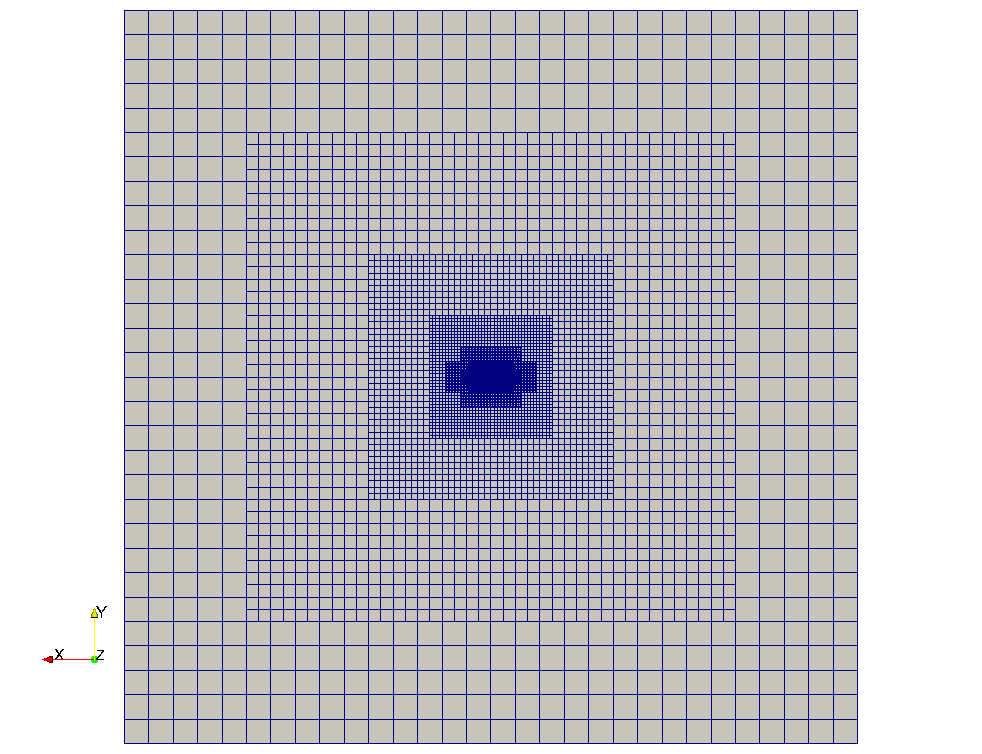
\includegraphics[width=.7\linewidth]{zoomedOutDemo1.png}
%  \caption{Zoomed out}
%  \label{fig:sub1}
%\\
%\end{subfigure}%
%\begin{subfigure}{\textwidth}
%  \centering
%  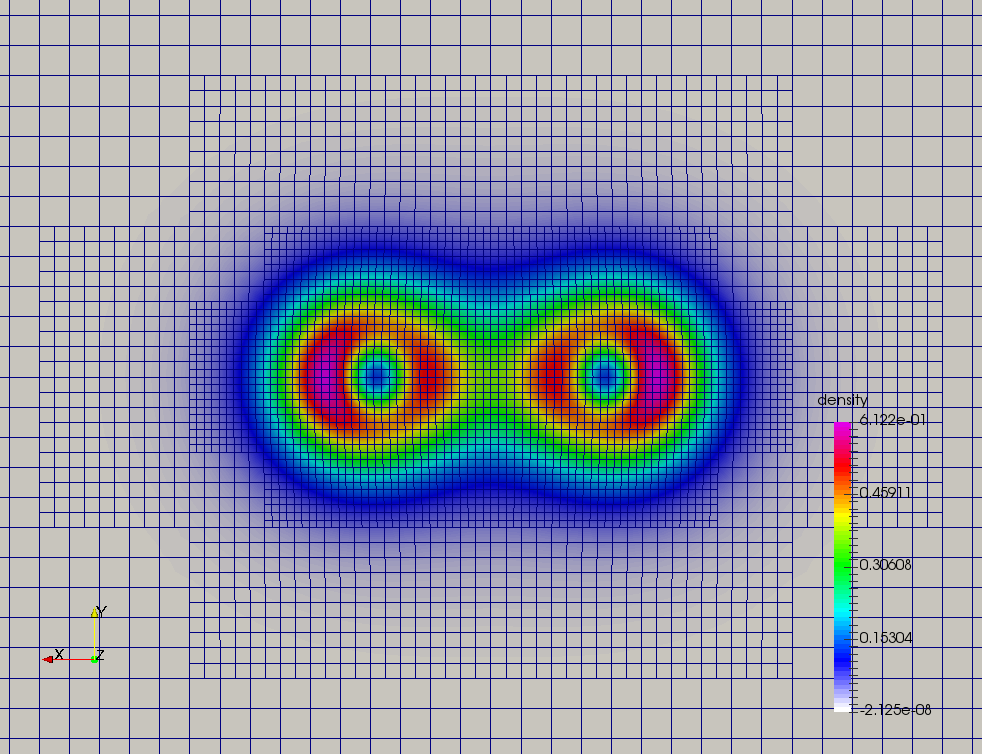
\includegraphics[width=.6\linewidth]{zoomedInDemo1.png}
%  \caption{Zoomed in with electron-density contours.}
%  \label{fig:sub2}
%\end{subfigure}
%	\caption{Finite-element mesh used in Nitrogen molecule pseudopotential DFT calculation (See \ref{sec:example1}).}
%\label{fig:N2}
%\end{figure}

\subsubsection{Example 2}\label{sec:example2}
In the previous example, we discussed how to setup and run a fully non-periodic problem.
Here we briefly discuss how to setup and run the fully periodic problem (FCC Aluminium unit cell) in the folder
\verb|/demo/ex2|. There are two input parameter files-- parameterFile\_a.prm and parameterFile\_b.prm. parameterFile\_a.prm is
for computing the ground-state and cell stress of the FCC Al unit cell, while parameterFile\_b.prm additionally does cell stress relaxation.  
Important input parameters in the above parameter files, beyond what we discussed in the previous example are
\begin{enumerate}
\item ``coordinates.inp'' given as input to \verb|ATOMIC COORDINATES FILE|, is the name of an external input file present in the same workspace which lists the fractional (reduced) coordinates of the atoms. For this example, ``coordinates.inp'' is described as 
\begin{verbatim}
13   3   0.00000000E+00   0.00000000E+00   0.00000000E+00
13   3   0.00000000E+00   0.50000000E+00   0.50000000E+00
13   3   0.50000000E+00   0.00000000E+00   0.50000000E+00
13   3   0.50000000E+00   0.50000000E+00   0.00000000E+00
\end{verbatim}
where each line corresponds to ``atomic-charge valence-charge fracx fracy fracz''. {\bf We require fractional coordinates for fully periodic or semi-periodic simulation domains while Cartesian coordinates are mandatory for fully non-periodic simulation domain.}
\item Set fully periodic boundary conditions
\begin{verbatim}	
subsection Boundary conditions
  set PERIODIC1                       = true
  set PERIODIC2                       = true
  set PERIODIC3                       = true
end
\end{verbatim}

\item Inside the \verb|Optimization| subsection, nested within the \verb|Geometry| subsection set 
\begin{verbatim}	
    set CELL STRESS = true
\end{verbatim}	
for computing the ground state cell stress. 

\item 
\begin{verbatim}
subsection Brillouin zone k point sampling options
  set USE TIME REVERSAL SYMMETRY = true
  subsection Monkhorst-Pack (MP) grid generation
    set SAMPLING POINTS 1 = 2
    set SAMPLING POINTS 2 = 2
    set SAMPLING POINTS 3 = 2
    set SAMPLING SHIFT 1  = 1
    set SAMPLING SHIFT 2  = 1
    set SAMPLING SHIFT 3  = 1
  end
end
\end{verbatim}
where
\begin{itemize}
\item \verb|SAMPLING POINTS 1/2/3| sets the number of Monkhorst-Pack grid points to be used along reciprocal lattice
vectors 1, 2, and 3.  		
\item Setting \verb|SAMPLING SHIFT 1/2/3| to 1 enables fractional shifting to be used along reciprocal lattice vectors.
\item Setting \verb|USE TIME REVERSAL SYMMETRY| to true enables use of time reversal symmetry to reduce number of k points to be solved for. For this option to work  \verb|SAMPLING SHIFT 1/2/3| must be set to 1 as done above. 
\end{itemize}

\item Set 
\begin{verbatim}	
subsection Parallelization
  set NPKPT=2
end
\end{verbatim}
which parallelizes the work load of the irreducible k-points across two groups of MPI tasks.

\item The same strategy for convergence of the ground state energy and force discussed
in the previous example is applied to the current example to get convergence in ground state energy and cell stress. 
The ground-state energy per atom and hydrostatic cell stress for finite-element meshes with increasing level of refinement is tabulated in Table~\ref{tab:table2}. Upon comparing the errors in the energy and force with respect the most refined mesh (\emph{Mesh No. 3}), we observe that for \emph{Mesh No. 1} we have obtained convergence in energy per atom to $\mathcal{O}(10^{-5})$ accuracy, and convergence in cell stress to $\mathcal{O}(10^{-7})$ accuracy.
\begin{table}[h!]
  \begin{center}
\small	  
    \caption{FCC Al ground-state energy and hydrostatic cell-stress convergence for demo example 2}
    \label{tab:table2}
    \begin{tabular}{c|c|c|c|c|c} 
	    % <-- Alignments: 1st column left, 2nd middle and 3rd right, with vertical lines in between
	    \hline\hline
	    Mesh No. &\verb|POLYNOMIAL| &\verb|MESH SIZE| & Total degrees of freedom& Energy per atom & Hydrostatic Cell stress\\
	    &\verb|ORDER| &\verb|AROUND ATOM| & per atom  & (Hartree) & (Hartree/${\rm Bohr}^3$) \\
      \hline
	    %1& 4 & 0.8 & 24,169  & -2.09083548 &  0.000028917\\	    
	    %2& 4 & 0.5 & 108,689 & -2.09322424 &  0.000037932\\
	    %3& 5 & 0.4 & 204,957 & -2.09322860 &  0.000038135\\
	    1& 5 & 1.6 & 4,394 & -2.30902819 &  -0.000109835\\	    
	    2& 5 & 1.3 & 7,447 & -2.30899310 &  -0.000110529\\
	    3& 6 & 1.3 & 12,663& -2.30900353 &  -0.000110531\\
       \hline\hline
    \end{tabular}
  \end{center}
\end{table}
The output file using the mesh parameters for \emph{Mesh No.1} is provided at \verb|/demo/ex2/ex2_a.output| (for parameterFile\_a.prm).

\item For cell stress relaxation, use parameterFile\_b.prm, where we set within the \verb|Optimization| subsection nested under \verb|Geometry|
\begin{verbatim}
    set STRESS TOL            = 4e-6
    set CELL OPT              = true
    set CELL CONSTRAINT TYPE  = 1
\end{verbatim}
where
\begin{itemize}
\item \verb|CELL OPT| is set to true which enables cell stress relaxation.  		
\item ``4e-6'' for \verb|STRESS TOL| sets the tolerance of the cell stress (in a.u.) for cell stress relaxation.
\item Choice of ``1'' for \verb|CELL CONSTRAINT TYPE| enforces isotropic shape-fixed volume optimization constraint during cell stress relaxation.
\end{itemize}
For your reference, the output file for the cell stress relaxation is provided at \verb|/demo/ex2/ex2_b.output|. From the output file, you should observe that you obtain a relaxed lattice constant of 7.699 Bohr after two geometry updates. You can also obtain the relaxed geometry from the \verb|domainBoundingVectorsCurrent.chk| file generated by the code.
\end{enumerate}

